
\definecolor{cebebeb}{RGB}{235,235,235}
\definecolor{c333333}{RGB}{51,51,51}
\definecolor{c4d4d4d}{RGB}{77,77,77}


\def \globalscale {1.000000}
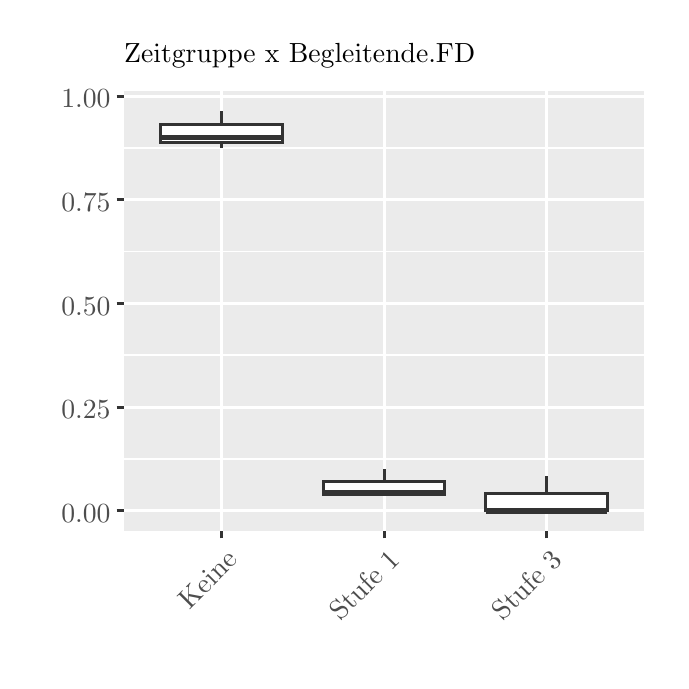
\begin{tikzpicture}[y=1mm, x=1mm, yscale=\globalscale,xscale=\globalscale, every node/.append style={scale=\globalscale}, inner sep=0pt, outer sep=0pt]
  \path[fill=white,line cap=round,line join=round,miter limit=10.0] ;



  \path[draw=white,fill=white,line cap=round,line join=round,line 
  width=0.38mm,miter limit=10.0] (0.0, 80.0) rectangle (80.0, 0.0);



  \path[fill=cebebeb,line cap=round,line join=round,line width=0.38mm,miter 
  limit=10.0] (12.07, 72.09) rectangle (78.07, 16.31);



  \path[draw=white,line cap=butt,line join=round,line width=0.19mm,miter 
  limit=10.0] (12.07, 25.43) -- (78.07, 25.43);



  \path[draw=white,line cap=butt,line join=round,line width=0.19mm,miter 
  limit=10.0] (12.07, 38.59) -- (78.07, 38.59);



  \path[draw=white,line cap=butt,line join=round,line width=0.19mm,miter 
  limit=10.0] (12.07, 51.76) -- (78.07, 51.76);



  \path[draw=white,line cap=butt,line join=round,line width=0.19mm,miter 
  limit=10.0] (12.07, 64.93) -- (78.07, 64.93);



  \path[draw=white,line cap=butt,line join=round,line width=0.38mm,miter 
  limit=10.0] (12.07, 18.85) -- (78.07, 18.85);



  \path[draw=white,line cap=butt,line join=round,line width=0.38mm,miter 
  limit=10.0] (12.07, 32.01) -- (78.07, 32.01);



  \path[draw=white,line cap=butt,line join=round,line width=0.38mm,miter 
  limit=10.0] (12.07, 45.18) -- (78.07, 45.18);



  \path[draw=white,line cap=butt,line join=round,line width=0.38mm,miter 
  limit=10.0] (12.07, 58.34) -- (78.07, 58.34);



  \path[draw=white,line cap=butt,line join=round,line width=0.38mm,miter 
  limit=10.0] (12.07, 71.51) -- (78.07, 71.51);



  \path[draw=white,line cap=butt,line join=round,line width=0.38mm,miter 
  limit=10.0] (24.44, 16.31) -- (24.44, 72.09);



  \path[draw=white,line cap=butt,line join=round,line width=0.38mm,miter 
  limit=10.0] (45.07, 16.31) -- (45.07, 72.09);



  \path[draw=white,line cap=butt,line join=round,line width=0.38mm,miter 
  limit=10.0] (65.69, 16.31) -- (65.69, 72.09);



  \path[draw=c333333,line cap=butt,line join=round,line width=0.38mm,miter 
  limit=10.0] (24.44, 67.9) -- (24.44, 69.56);



  \path[draw=c333333,line cap=butt,line join=round,line width=0.38mm,miter 
  limit=10.0] (24.44, 65.58) -- (24.44, 64.93);



  \path[draw=c333333,fill=white,line cap=butt,line join=miter,line 
  width=0.38mm,miter limit=10.0] (16.71, 67.9) -- (16.71, 65.58) -- (32.18, 
  65.58) -- (32.18, 67.9) -- (16.71, 67.9) -- (16.71, 67.9)-- cycle;



  \path[draw=c333333,line cap=butt,line join=miter,line width=0.75mm,miter 
  limit=10.0] (16.71, 66.24) -- (32.18, 66.24);



  \path[draw=c333333,line cap=butt,line join=round,line width=0.38mm,miter 
  limit=10.0] (45.07, 22.57) -- (45.07, 24.11);



  \path[draw=c333333,line cap=butt,line join=round,line width=0.38mm,miter 
  limit=10.0] (45.07, 20.92) -- (45.07, 20.8);



  \path[draw=c333333,fill=white,line cap=butt,line join=miter,line 
  width=0.38mm,miter limit=10.0] (37.33, 22.57) -- (37.33, 20.92) -- (52.8, 
  20.92) -- (52.8, 22.57) -- (37.33, 22.57) -- (37.33, 22.57)-- cycle;



  \path[draw=c333333,line cap=butt,line join=miter,line width=0.75mm,miter 
  limit=10.0] (37.33, 21.04) -- (52.8, 21.04);



  \path[draw=c333333,line cap=butt,line join=round,line width=0.38mm,miter 
  limit=10.0] (65.69, 21.04) -- (65.69, 23.23);



  \path[draw=c333333,line cap=butt,line join=round,line width=0.38mm,miter 
  limit=10.0] ;



  \path[draw=c333333,fill=white,line cap=butt,line join=miter,line 
  width=0.38mm,miter limit=10.0] (57.96, 21.04) -- (57.96, 18.85) -- (73.43, 
  18.85) -- (73.43, 21.04) -- (57.96, 21.04) -- (57.96, 21.04)-- cycle;



  \path[draw=c333333,line cap=butt,line join=miter,line width=0.75mm,miter 
  limit=10.0] (57.96, 18.85) -- (73.43, 18.85);



  \node[text=c4d4d4d,anchor=south east] (text4633) at (10.33, 17.33){0.00};



  \node[text=c4d4d4d,anchor=south east] (text9798) at (10.33, 30.5){0.25};



  \node[text=c4d4d4d,anchor=south east] (text8310) at (10.33, 43.67){0.50};



  \node[text=c4d4d4d,anchor=south east] (text7477) at (10.33, 56.83){0.75};



  \node[text=c4d4d4d,anchor=south east] (text1611) at (10.33, 70.0){1.00};



  \path[draw=c333333,line cap=butt,line join=round,line width=0.38mm,miter 
  limit=10.0] (11.1, 18.85) -- (12.07, 18.85);



  \path[draw=c333333,line cap=butt,line join=round,line width=0.38mm,miter 
  limit=10.0] (11.1, 32.01) -- (12.07, 32.01);



  \path[draw=c333333,line cap=butt,line join=round,line width=0.38mm,miter 
  limit=10.0] (11.1, 45.18) -- (12.07, 45.18);



  \path[draw=c333333,line cap=butt,line join=round,line width=0.38mm,miter 
  limit=10.0] (11.1, 58.34) -- (12.07, 58.34);



  \path[draw=c333333,line cap=butt,line join=round,line width=0.38mm,miter 
  limit=10.0] (11.1, 71.51) -- (12.07, 71.51);



  \path[draw=c333333,line cap=butt,line join=round,line width=0.38mm,miter 
  limit=10.0] (24.44, 15.34) -- (24.44, 16.31);



  \path[draw=c333333,line cap=butt,line join=round,line width=0.38mm,miter 
  limit=10.0] (45.07, 15.34) -- (45.07, 16.31);



  \path[draw=c333333,line cap=butt,line join=round,line width=0.38mm,miter 
  limit=10.0] (65.69, 15.34) -- (65.69, 16.31);



  \node[text=c4d4d4d,anchor=south east,cm={ 0.71,0.71,-0.71,0.71,(26.58, 
  -67.57)}] (text8032) at (0.0, 80.0){Keine};



  \node[text=c4d4d4d,anchor=south east,cm={ 0.71,0.71,-0.71,0.71,(47.21, 
  -67.57)}] (text892) at (0.0, 80.0){Stufe 1};



  \node[text=c4d4d4d,anchor=south east,cm={ 0.71,0.71,-0.71,0.71,(67.83, 
  -67.57)}] (text1336) at (0.0, 80.0){Stufe 3};



  \node[anchor=south west] (text3678) at (12.07, 75.04){Zeitgruppe x 
  Begleitende.FD};




\end{tikzpicture}
